\documentclass[10pt]{beamer}

\usetheme[progressbar=frametitle]{metropolis}
\usepackage{appendixnumberbeamer}

\usepackage{booktabs}
\usepackage[scale=2]{ccicons}

\usepackage{pgfplots}
\usepgfplotslibrary{dateplot}

\usepackage{xspace}
\newcommand{\themename}{\textbf{\textsc{metropolis}}\xspace}

\usepackage{graphicx}
\graphicspath{ {pics/} }

\usepackage{listings}
\definecolor{mGreen}{rgb}{0,0.6,0}
\definecolor{mGray}{rgb}{0.5,0.5,0.5}
\definecolor{mPurple}{rgb}{0.58,0,0.82}
\definecolor{backgroundColour}{rgb}{0.95,0.95,0.92}

\lstdefinestyle{CStyle}{
    backgroundcolor=\color{backgroundColour},
    commentstyle=\color{mGreen},
    keywordstyle=\color{magenta},
    numberstyle=\tiny\color{mGray},
    stringstyle=\color{mPurple},
    basicstyle=\footnotesize,
    breakatwhitespace=false,
    %breaklines=true,
    captionpos=b,
    keepspaces=true,
    %numbers=left,
    numbersep=5pt,
    showspaces=false,
    showstringspaces=false,
    showtabs=false,
    tabsize=2,
    language=C
}

\lstdefinestyle{HTMLStyle}{
    backgroundcolor=\color{backgroundColour},
    commentstyle=\color{mGreen},
    keywordstyle=\color{magenta},
    numberstyle=\tiny\color{mGray},
    stringstyle=\color{mPurple},
    basicstyle=\tiny,
    breakatwhitespace=false,
    breaklines=true,
    captionpos=b,
    keepspaces=true,
    numbersep=5pt,
    showspaces=false,
    showstringspaces=false,
    showtabs=false,
    tabsize=2,
    language=HTML
}

\lstdefinestyle{BashStyle}{
    backgroundcolor=\color{backgroundColour},
    commentstyle=\color{mGreen},
    keywordstyle=\color{magenta},
    numberstyle=\tiny\color{mGray},
    stringstyle=\color{mPurple},
    basicstyle=\footnotesize,
    breakatwhitespace=false,
    %breaklines=true,
    captionpos=b,
    keepspaces=true,
    %numbers=left,
    numbersep=5pt,
    showspaces=false,
    showstringspaces=false,
    showtabs=false,
    tabsize=2,
    language=Bash
}

%----------------------------------------------------------------------------------------
%	TITLE PAGE
%----------------------------------------------------------------------------------------

\title{Software Security}
\subtitle{Kryptographie und IT Sicherheit SS 2018}
% \date{\today}
\date{}
\author{Dmitrii Polianskii, Manuel Klappacher}
\institute{Universit\"at Salzburg}
% \titlegraphic{\hfill
\includegraphics[height=1.5cm]{logo.pdf}}

\begin{document}

\maketitle

\begin{frame}{Themen}
  \setbeamertemplate{section in toc}[sections numbered]
  \tableofcontents[hideallsubsections]
\end{frame}

%----------------------------------------------------------------------------------------
%	Einleitung
%----------------------------------------------------------------------------------------

\section{Einleitung}

\begin{frame}[fragile]{Wie entstehen Fehler und Sicherheitsl\"ucken?}
  \begin{itemize}
    \item Programmierfehler
      \begin{itemize}
        \item Treten sehr h\"aufig auf
        \item Logische Fehler, syntaktische Fehler, lexikalische Fehler
        \item Zeitdruck
        \item Mangelnde Kenntniss
        \item Keine ausreichenden Tests
      \end{itemize}
    \item Compilerfehler
      \begin{itemize}
        \item Treten nicht sehr h\"aufig auf
      \end{itemize}
    \item Absichtlich platzierte Backdoors
      \begin{itemize}
        \item Sehr schwer nachzuweisen - wie Unterscheidet man Fehler von b\"oswilliger Absicht?
        \item Werden auch von anderen Teilnehmern entdeckt und von Kriminellen dann f\"ur ihre Zwecke missbraucht
      \end{itemize}
    \item Zuviel Komplexit\"at
      \begin{itemize}
        \item Komplexe Systeme kann keiner mehr \"uberblicken
        \item schwer \"uber Sicherheit argumentierbar
      \end{itemize}
  \end{itemize}
\end{frame}

%----------------------------------------------------------------------------------------
%	REMOTE AND LOCAL THREATS
%----------------------------------------------------------------------------------------

\section{Remote and Lokale Gefahren}

\begin{frame}[fragile]{Einleitung - Statistiken}
  Most commonly exploited applications worldwide as of 3rd quarter 2017
  \newline
  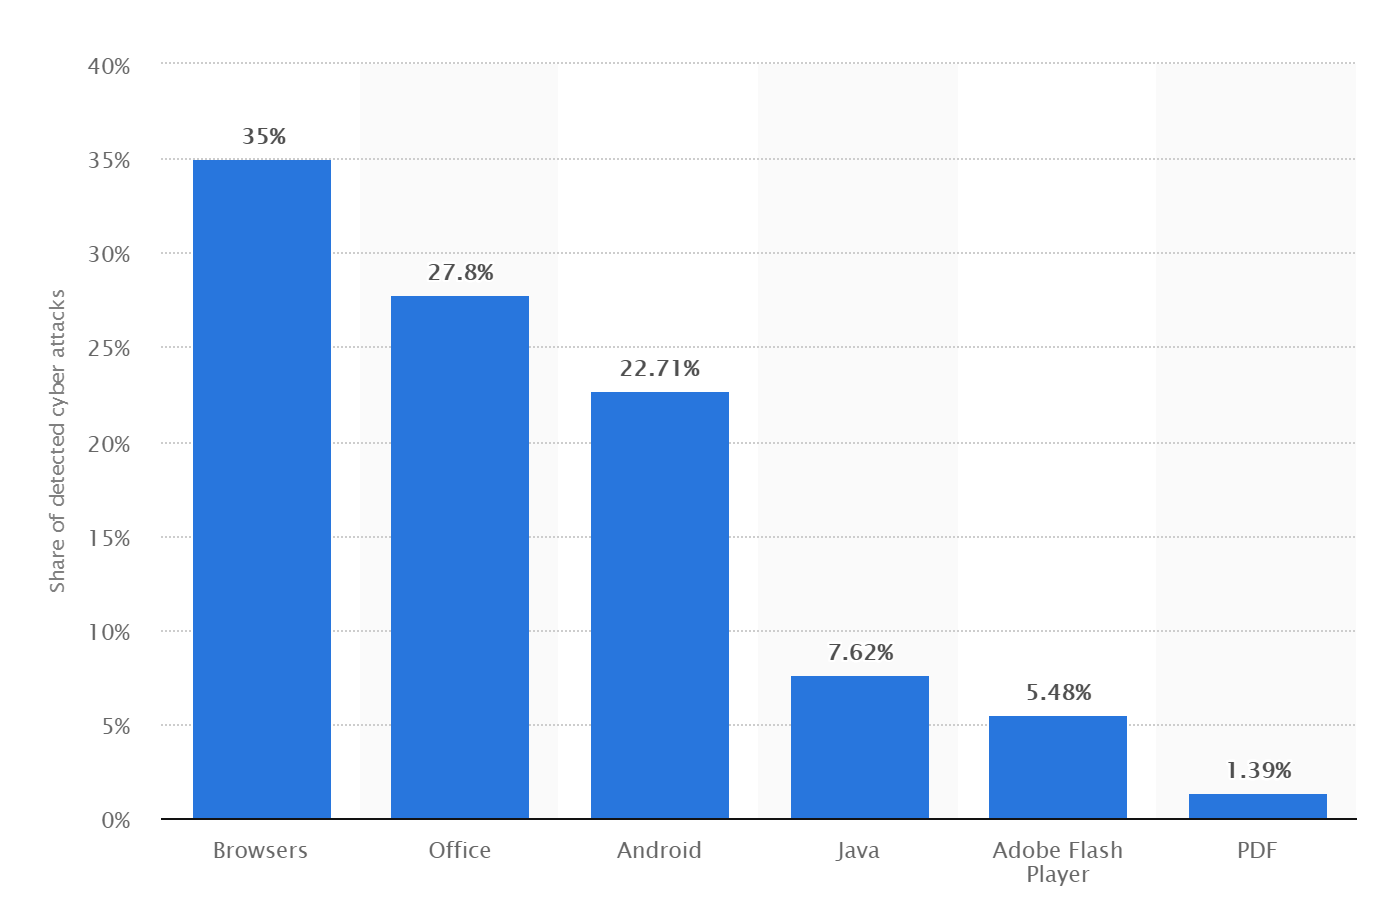
\includegraphics[scale=0.5]{cyberattacks_2017}
  \newline
  Quelle: www.statista.com
\end{frame}


%----------------------------------------------------------------------------------------
%	EXPLOITS
%----------------------------------------------------------------------------------------

\section{Exploits}

\begin{frame}[fragile]{Code Injection}
  Code Injection ist das ausnutzen von Bugs durch Eingabe von ungewollten Parametern, um dadurch die Ausf\"urung zu ver\"andern.
  \newline
  Kann folgende Auswirkungen haben:
  \begin{itemize}
    \item Daten in SQL Tabellen ver\"andern
    \item Installieren von Malware durch Server-Scripting Code zB. PHP
    \item Root Privilegien bekommen, durch Shell Injection oder Windows Service
    \item Angtiff auf Web User durch Cross-Site-Scripting in HTML/JS
  \end{itemize}
\end{frame}

\begin{frame}[fragile]{Code Injection - Masnahmen}
  Kann erschwert werden durch:
  \begin{itemize}
    \item API's benutzen, die sicher gegen\"uber allen Symbolen sind, indem der Eingabestring compiliert und gefiltert wird.
    \item Whitelisting von erw\"unschten Parametern
  \end{itemize}
\end{frame}

\begin{frame}[fragile]{SQL Injection}
  Ausnutzen von Sicherheitsl\"ucken in Zusammenhang mit SQL-Datenbanken.
  Ziele:
  \begin{itemize}
    \item Daten auszusp\"ahen oder zu ver\"andern
    \item Kontrolle \"uber Server zu erhalten
  \end{itemize}
\end{frame}

\begin{frame}[fragile]{SQL Injection - Beispiel}
  Es wird zus\"atzlicher Code bei Aufruf eingeschleust, der die Benutzertabelle modifiziert.
  \newline
  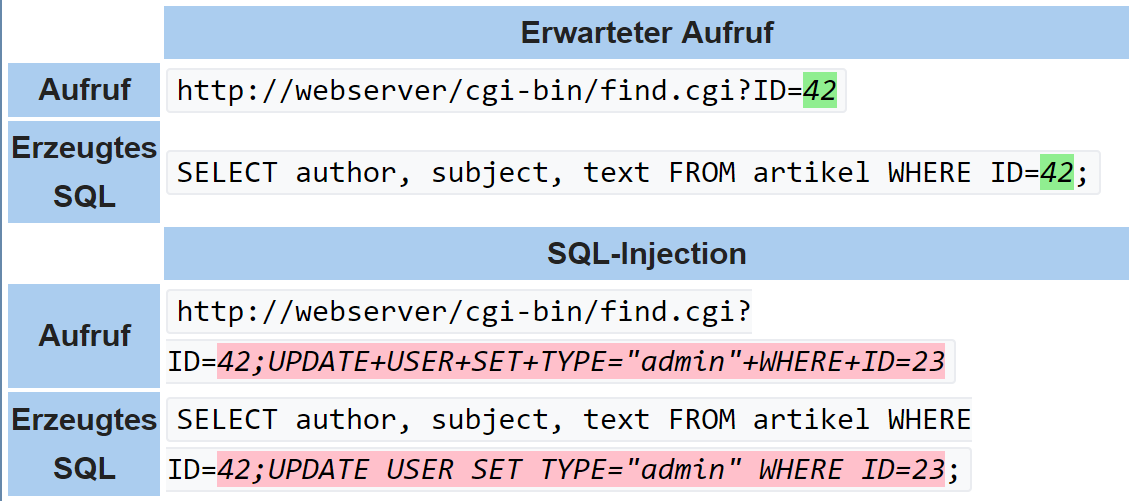
\includegraphics[scale=0.5]{sql_injection_1}
\end{frame}

\begin{frame}[fragile]{Cross Site Scripting - XSS}
  Bei Cross-Site Scripting (XSS) werden Sicherheitsl\"ucken in Webanwendungen ausgenutzt um schadhaften Code in sonst vertrauensw\"urdigen Websiten einzubinden.
  Das ist der Fall wenn es nicht Vertrauensw\"urdigen Dritten erlaubt ist, Daten und Code hochzuladen.
  \newline
  Ziele:
  \begin{itemize}
    \item Benutzerkonten zu \"ubernehmen
    \item Daten (Identit\"atsdiebstahl)
  \end{itemize}
  Der Browser des Benutzers kann nicht zwischen sch\"adlichem und gew\"unschtem Code unterscheiden.
\end{frame}

\begin{frame}[fragile]{Cross Site Scripting - reflektierte Angriffe}
  Eine Benutzereingabe wird direkt vom Server wieder zur\"uck gesendet.
  Wenn diese Eingabe Scriptcode enth\"alt, die vom Browser des Nutzers interpretiert wird, kann dort Schadcode ausgef\"urt werden.
  Beispiel: Suchfunktion.
  \begin{lstlisting}[style=CStyle]
    http://example.com/?suche=Suchbegriff

    http://example.com/?suche=<script type=
          "text/javascript">alert("XSS")</script>

    <p>Sie suchten nach: <script type=
          "text/javascript">alert("XSS")</script></p>
  \end{lstlisting}
  Ausgenutzt wird das dynamisch generierte Websiten ihren Ihnalt an \"ubergebene Eingabewerte anpassen, durch HTTP-GET und HTTP-POST.
  Dieser Typ heisst auch nicht-persistent, da der Schadcode nur tempr\"ar bei der jeweiligen Generierung der Website eingeschleust wird.
\end{frame}

\begin{frame}[fragile]{Cross Site Scripting - persistente Angriffe}
  Unterscheidet sich von reflektierenden Angriffen nur dadurch, dass der Schadcode auf dem Server gespeichert wird, wodurch er bei jeder Anfrage asugef\"urt wird.
  Ist bei Webanwendungen m\"oglich, die Benutzereingaben serverseitig ohne Pr\"ufung speichern und diese sp\"ater wieder ausliefert.
  Beispiel Posting auf Website:
  \begin{lstlisting}[style=CStyle]
    Eine sehr gutes Produkt!<script type=
          "text/javascript">alert("XSS")</script>
  \end{lstlisting}
\end{frame}

\begin{frame}[fragile]{Cross Site Scripting - DOM-basierte Angriffe}
  Webapplikation auf dem Server ist hier nicht beteiligt, wird auch lokales XSS genannt.
  Somit auch statische HTML Seiten mit JavaScript unterst\"utzung anf\"allig f\"ur diesen Angriff.
\end{frame}

\begin{frame}[fragile]{Cross Site Scripting - Schutzma{\ss}nahmen}
  \begin{itemize}
    \item Anstatt Blacklist mit b\"osen Eingaben zu f\"uhren, besser Whitelist mit buten Eingaben. Da die Anzahl der Angriffmethoden nicht bekannt ist.
    \item HTML-Metazeichen durch Zeichenreferenzen ersetzen, damit sie als normale Zeichen behandelt werden
    \item Sicher programmierte Anwendung sind Web Apllication Firewalls (WAF) vorzuziehen.
  \end{itemize}
\end{frame}

\begin{frame}[fragile]{Directory Traversal Attack}
  Ein HTTP Angriff, bei dem ein Angreifer zugriff auf gesperrte Verzeichnisse gewinnt und Code auserhalb des root Verzeichnisses ausf\"uhrt.
\end{frame}

\begin{frame}[fragile]{Directory Traversal Attack - Schutzma{\ss}nahmen}
  test frame
\end{frame}

\begin{frame}[fragile]{Format String}
  Format Funktion ist eine ANSI C Funktion, um primitive Variablen in eine lesbare Ausgabe konvertieren. z.B. \textit{printf}, \textit{fprintf}
  \begin{itemize}
    \item Sind C/C++ Probleme
    \item treten heute nicht sehr h\"afig auf, da sie sich sehr leicht erkennen lassen
  \end{itemize}
  Ziele:
  \begin{itemize}
    \item Programmcrash
    \item Schadcode ausf\"uhrung
  \end{itemize}
\end{frame}

\begin{frame}[fragile]{Format String - Beispiel I}

  \begin{lstlisting}[style=CStyle]
  int main (int argc, char **argv)
  {
	   char buf [100];
	   int x = 1 ;

	   snprintf ( buf, sizeof buf, argv [1] ) ;
	   buf [ sizeof buf -1 ] = 0;

	   printf ( “Buffer size is: (%d)
          \nData input: %s \n” , strlen (buf) , buf ) ;

	   printf ( “X equals: %d/ in
          hex: %#x\nMemory address
          for x: (%p) \n” , x, x, &x) ;

	   return 0 ;
  }
  \end{lstlisting}
\end{frame}

\begin{frame}[fragile]{Format String - Beispiel II}
  Erwartete Eingabe:
  \begin{lstlisting}[style=BashStyle]
  ./formattest “Bob”
  \end{lstlisting}
  Ausgabe:
  \begin{lstlisting}[style=BashStyle]
  Buffer size is (3)
  Data input : Bob
  X equals: 1/ in hex: 0x1
  Memory address for x (0xbffff73c)
  \end{lstlisting}
\end{frame}

\begin{frame}[fragile]{Format String - Beispiel III}
  Schwachstelle ausgenutzt, \%x := Ausgabe Hexadezimal:
  \begin{lstlisting}[style=BashStyle]
  ./formattest “Bob %x %x”
  \end{lstlisting}
  Anstatt \%x Wert von Bob auszugeben, gibt nun auch den Inhalt der Speicher Adresse aus:
  \begin{lstlisting}[style=BashStyle]
  Buffer size is (14)
  Data input : Bob bffff 8740
  X equals: 1/ in hex: 0x1
  Memory address for x (0xbffff73c)
  \end{lstlisting}

  \textit{printf} Argument sieht nun folgenderma{\ss}en aus:
  \begin{lstlisting}[style=CStyle]
  printf ( “Buffer size is: (%d) \n Data input:
      Bob %x %x \n” , strlen (buf) , buf ) ;
  \end{lstlisting}
\end{frame}

\begin{frame}[fragile]{Buffer Overflows}
  Durch Programmfehler werden zu gro{\ss}e Datenmengen in einen zu klein reservierten Speicherbereich geschrieben.
  (Buffer oder Stack, auch Pointer).
  \newline
  \newline
  $\rightarrow$ Daten werden \"uberschrieben:
  \begin{itemize}
    \item Schadcode wird ausgef\"uhrt
    \item Absturz des Programms
    \item Besch\"adigung oder Verf\"alschung von Daten
  \end{itemize}
  Zum Beispiel die R\"ucksprungadresse eines Unterprogrammes wird \"uberschrieben.
\end{frame}

\begin{frame}[fragile]{Buffer Overflows}
  Beg\"unstigt durch Van Neumann Architektur, Daten und Programm im selben Speicher.
  \begin{itemize}
    \item Compilierte und assemblierte Sprachen anf\"allig
    \item Anf\"allige Sprachen, z.B. C/C++
    \item Unsichere Libraries in C/C++
    \item Unsicheres Behandeln von Stirngs und Arraygr\"o{\ss}en
  \end{itemize}
  Schutzma{\ss}nahmen:
  \begin{itemize}
    \item Type-Safe Programmiersprachen verwenden, welche Memory Management zB Java, Python, Ruby,...
    \item \"Uberpr\"ufen auf Overflows bei User Eingaben
    \item in C sichere Methoden verwenden, \textit{get\_s} anstatt \textit{get}.
  \end{itemize}
\end{frame}

\begin{frame}[fragile]{Buffer Overflows - Type-Safe Sprachen}
  Compiler stellt Typsicherheit her, indem Datentypen gepr\"uft werden, damit keine Typverletzungen entstehen.
  Wenn Typverletzungen sp\"atestens zur Laufzeit erkannt werden, spricht man von Typsicheren Programmiersprachen.

  Beispiel String in Python, es reicht der Variable einen String zuzuweisen.
  \begin{lstlisting}[style=CStyle]
    mystring = "This is my string"
  \end{lstlisting}

  Beispiel in C, es muss der Typ deklariert und auch der Speicher manuell reserviert werden.
  \begin{lstlisting}[style=CStyle]
    char mystring[20] = "This is my string";
  \end{lstlisting}
  Wenn man in C nun einen 30 Byte String zuweist entsteht eine Overflow Situation.
\end{frame}

\begin{frame}[fragile]{Buffer Overflows - Stack Overflow}
 Die R\"ucksprungadresse eines Unterprogramms und dessen lokale Variablen werden auf einen als Stack bezeichneten Bereich zu gelegt.
 \begin{lstlisting}[style=CStyle]
  void input_line()
  {
    char line[1000];
    if (gets(line))
      puts(line);
  }
 \end{lstlisting}

 \begin{figure}%
  \centering
  {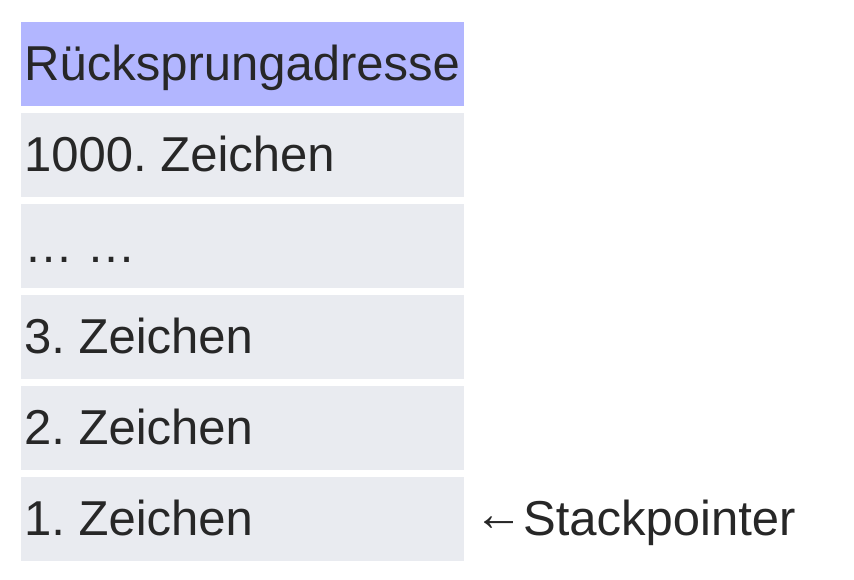
\includegraphics[scale=0.10]{stackoverflow}}%
  \quad
  {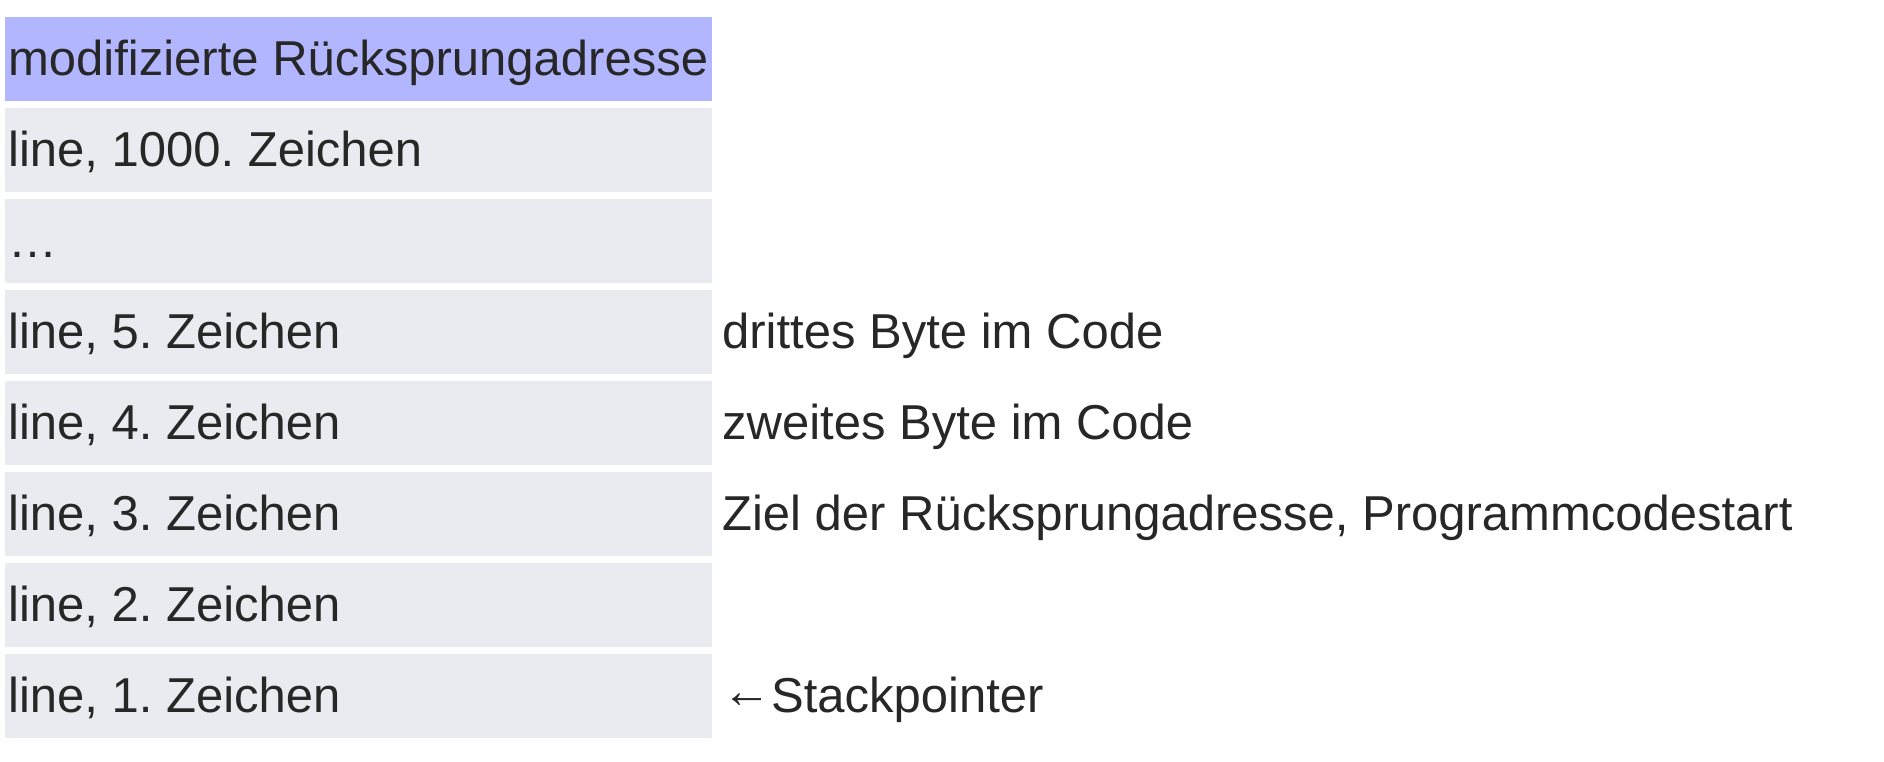
\includegraphics[scale=0.10]{stackoverflow_2}}%
 \end{figure}
\end{frame}

\begin{frame}[fragile]{Buffer Overflows - Compiler Ma{\ss}nahmen}
  Moderne Compiler wie neue Versionen des GNU C-Compilers erlauben die Aktivierung von \"Uberpr\"ufungscode-Erzeugung bei der \"Ubersetzung.

  \begin{itemize}
    \item Zufallsvariable erstellt und \"uberpr\"uft, bei Ver\"anderung wurde auch die RA \"uberschrieben.
    \item Kopie der R\"ucksprungadresse wird unterhalb lokaler Variablen abgelegt.
  \end{itemize}

  \begin{figure}%
   \centering
   {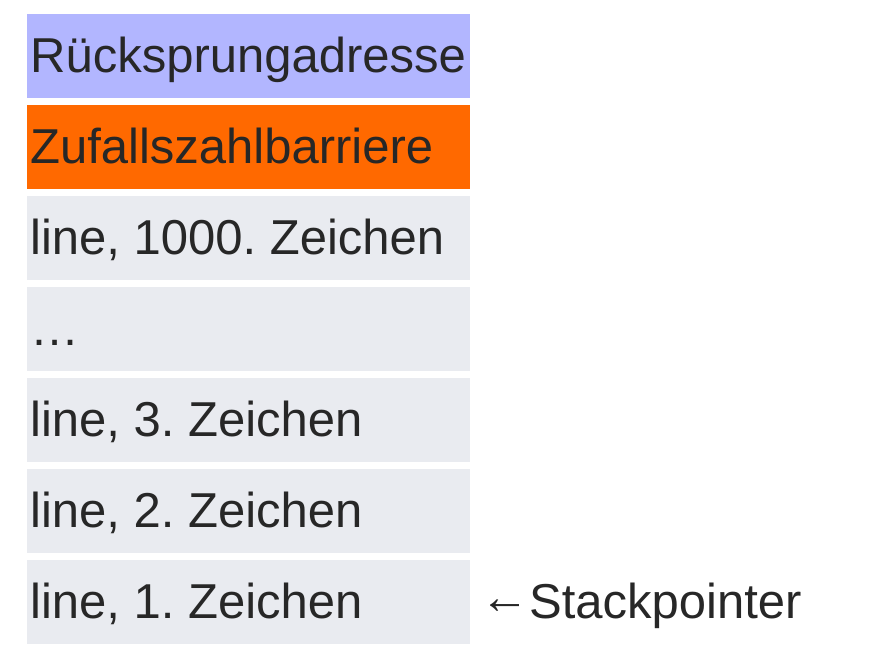
\includegraphics[scale=0.10]{stackgcc_1}}%
   \quad
   {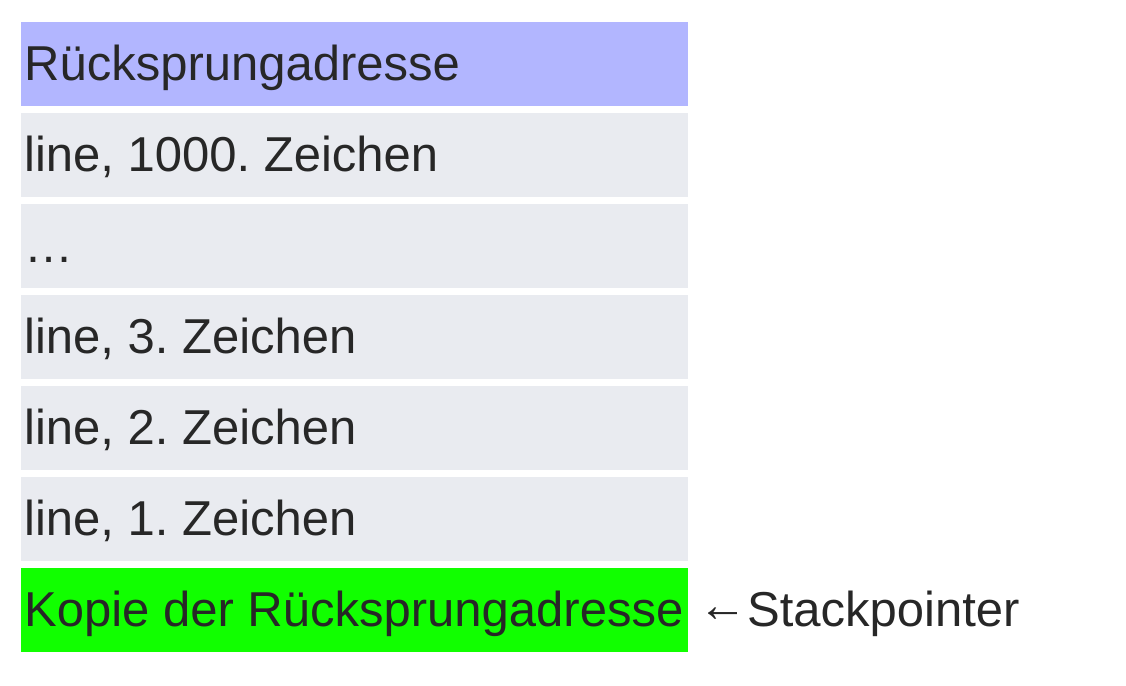
\includegraphics[scale=0.10]{stackgcc_2}}%
  \end{figure}
\end{frame}

\begin{frame}[fragile]{Buffer Overflows - Programmbeispiel}
  reserved frame
\end{frame}

\begin{frame}[fragile]{Buffer Overflows - Heap Overflows}
  Ist ein Buffer Overflow, der im Heap Bereich stattfindet.
  \begin{itemize}
    \item Daten werden zur Laufzeit gespeichert (malloc)
    \item Kein Limit, ausser RAM Gr\"o{\ss}e
    \item in iOS Jailbreaks verwenden Heap Overflows um Code in den Kernel zu injizieren
  \end{itemize}
  Gegenma{\ss}nahmen:
  \begin{itemize}
    \item Code und Daten trennen mit Prozessoren - NX-bit - No Execute Bit
    \item Betriebssysteme mit ASLR - Address Space Layout Randomization
    \item Checks im Heap Manager
  \end{itemize}
\end{frame}

\begin{frame}[fragile]{Integer Overflows}
  Entstehen wenn Operationen auf Integer die maximale Gr\"o{\ss}e \"uberschreiten. z.B. arithemetische oder cast Operationen.
  \begin{itemize}
    \item testen ob Maximaler Wert \"uberschritten ist
    \item Typen beachten, signed unsigned
    \item muss von Hand gemacht werden, keine nativen Methoden in Programmiersprachen
    \item in Java BigInt verwenden
  \end{itemize}
  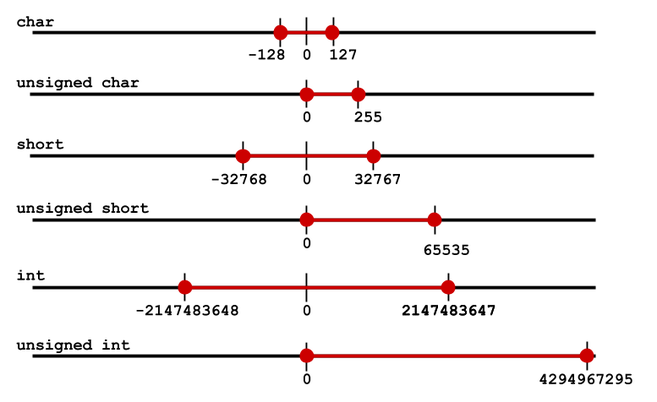
\includegraphics[scale=0.25]{integer_overflow}
\end{frame}

%----------------------------------------------------------------------------------------
%	OPEN SOURCE UND PROPERTÄRE SOFTWARE
%----------------------------------------------------------------------------------------

\section{Open Source und Propert\"are Software}

\begin{frame}[fragile]{Open Source Vorteile}
  \begin{itemize}
    \item Programmcode kann \"uberpr\"uft werden, Sicherheitsl\"ucken fallen leichter auf
    \item Erschwert implementierung von Backdoors
    \item Software kann von der Communtiy weiterentwickelt oder geforkt werden
    \item Bestimmte Funktionen k\"onnen abgedreht werden
  \end{itemize}
\end{frame}

%----------------------------------------------------------------------------------------
%	FIRMWARE SECURITY
%----------------------------------------------------------------------------------------

\section{Firmware Security}
\begin{frame}[fragile]{Spezialfall Firmware}
  \begin{itemize}
    \item Ger\"at wurde bereits verkauft, kein Interesse des Herstellers an Updates
    \item Zu viele verschiedene Ger\"ate - Unm\"oglicher Verwaltungsaufwand
      \begin{itemize}
        \item Alleine Samsung hat bis 2014 56 verscheidene Smartphones pro Jahr herausgebracht
      \end{itemize}
    \item Firmware agiert in Schicht unter Betriebssystem - Angriffe k\"onnen vom Benutzer nicht erkannt oder verhindert werden
    \item Firmware meist Closed Source - keine Weiterentwicklung der Community
  \end{itemize}
\end{frame}

\begin{frame}[fragile]{Sicherheitsl\"ucken in Firmware - Beispiele}
  \begin{itemize}
    \item BadUSB - Eingabeger\"ate, USB-Sticks, Speichermedien, Kameras, ...
    \item Intel ME - Betriebssystem im Prozessor (AMD PSP)
      \begin{itemize}
        \item Funktionsweise undokumentiert
        \item Kritische L\"ucke 2017 entdeckt
        \item NSA und Google haben Intel ME abgeschaltet auf ihren Ger\"aten
      \end{itemize}
    \item Android
      \begin{itemize}
        \item praktisch alle Android Ger\"ate ohne Sicherheitupdates
      \end{itemize}
    \item Router, Smart TV's, IoT-Devices - Millionen angreifbare Ger\"ate in Haushalten, Firmen und Beh\"orden
  \end{itemize}
\end{frame}

\begin{frame}[fragile]{Smartphones Sicherheitsupdates}
  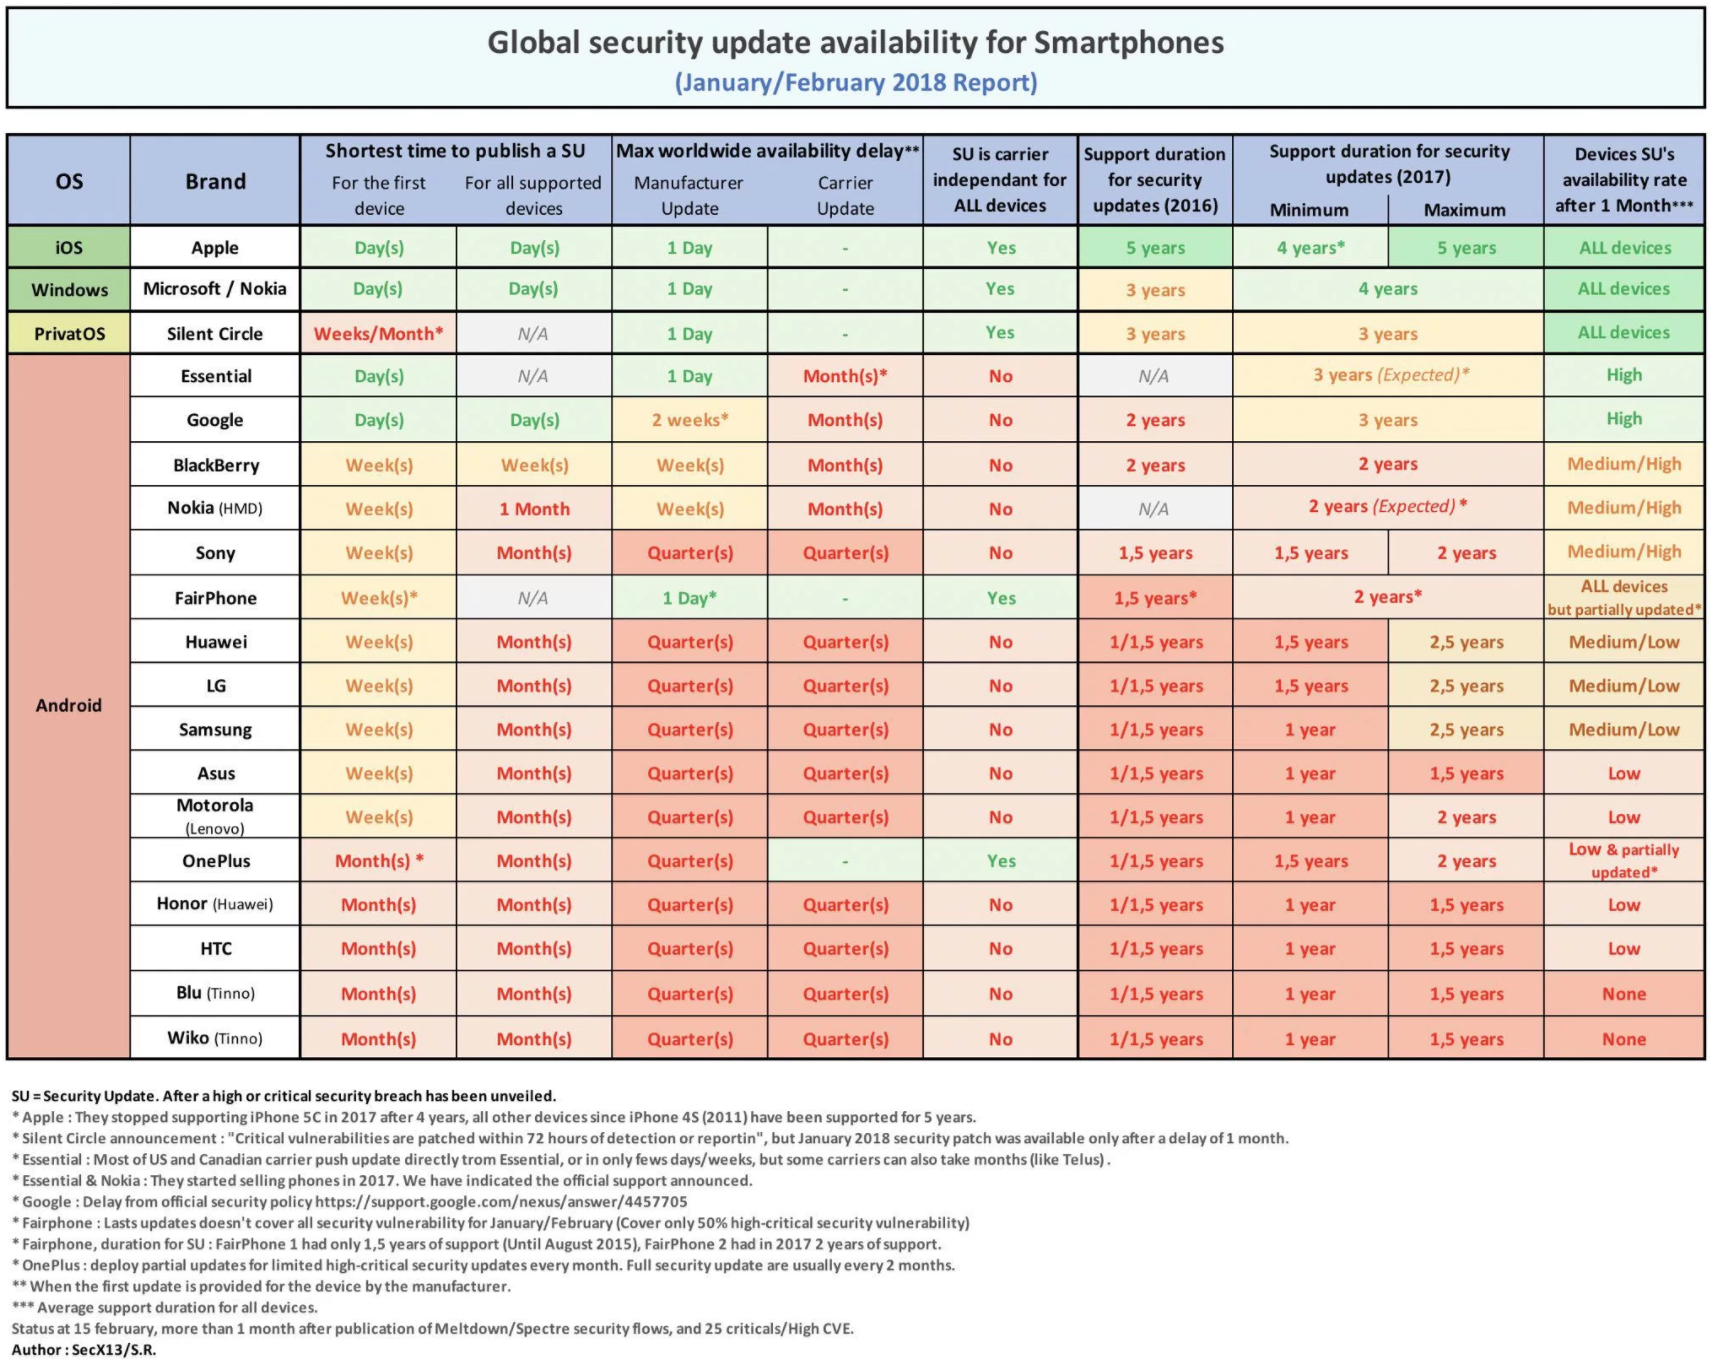
\includegraphics[scale=0.5]{android_sub}
  \newline
\end{frame}

\begin{frame}[fragile]{Quellen}
  \begin{itemize}
    \item wikipedia.org
    \item owasp.org
  \end{itemize}
\end{frame}

\begin{frame}[fragile]{}
  \huge Vielen Dank f\"ur ihre Aufmerksamkeit!
\end{frame}

\end{document}
